\documentclass[11pt]{article}
\usepackage[a4paper,margin=1in]{geometry}
\usepackage[T1]{fontenc}
\usepackage[expansion=false]{microtype}
\usepackage{amsmath,amssymb,amsthm}
\usepackage{booktabs,longtable,array}
\usepackage{graphicx}
\usepackage[font=small,labelfont=bf]{caption}
\usepackage[authoryear,round]{natbib}
\usepackage[dvipsnames]{xcolor}
\usepackage[colorlinks=true,linkcolor=blue!60!black,citecolor=blue!60!black,urlcolor=blue!60!black]{hyperref}
\usepackage{enumitem}
\usepackage{needspace}
\usepackage[section]{placeins}
\setlist{nosep,leftmargin=1.5em}
\newcommand{\bpcMin}{2.325}
\newcommand{\bpcMax}{2.394}
\newcommand{\bpcRange}{0.068}
\newcommand{\uniformBpc}{2.929}
\newcommand{\attnEffect}{0.54}
\newcommand{\lpMin}{2.333}
\newcommand{\lpMax}{2.394}
\newcommand{\rangeFraction}{11}
\newcommand{\tiedDtwo}{2.344}
\newcommand{\tiedDsixteen}{2.338}
\newcommand{\untiedDsixteen}{2.325}
\newcommand{\unmaskedDsixteen}{2.329}
\newcommand{\medianSeedSd}{0.0096}
\newcommand{\minSeedSd}{0.0034}
\newcommand{\maxSeedSd}{0.0267}
\newcommand{\spreadPTwo}{0.014}
\newcommand{\spreadPFour}{0.009}
\newcommand{\spreadPEight}{0.016}
\newcommand{\spreadPTwelve}{0.015}
\newcommand{\spreadPSixteen}{0.031}
\newcommand{\nPositive}{34}
\newcommand{\nHolm}{15}
\newcommand{\nHolmTwo}{7}
\newcommand{\nHolmOther}{8}
\newcommand{\nHolmFour}{3}
\newcommand{\nHolmEight}{2}
\newcommand{\nHolmTwelve}{2}
\newcommand{\nHolmSixteen}{1}
\newcommand{\nUncorr}{24}
\newcommand{\nNegative}{1}
\newcommand{\gapTwoMin}{0.036}
\newcommand{\gapTwoMax}{0.050}
\newcommand{\gapOtherMedian}{0.016}
\newcommand{\gapOtherMin}{-0.005}
\newcommand{\gapOtherMax}{0.028}
\newcommand{\exceptionGap}{-0.005}
\newcommand{\exceptionP}{0.26}
\newcommand{\exceptionCIlo}{-0.016}
\newcommand{\exceptionCIhi}{0.005}
\newcommand{\untiedMin}{-0.013}
\newcommand{\untiedMax}{-0.004}
\newcommand{\untiedEightP}{0.012}
\newcommand{\untiedEight}{-0.011}
\newcommand{\untiedSixteen}{-0.013}
\newcommand{\untiedSixteenP}{0.069}
\newcommand{\maskDiff}{0.003}
\newcommand{\maskLo}{-0.013}
\newcommand{\maskHi}{0.020}
\newcommand{\maskP}{0.61}
\newcommand{\slopeMean}{-0.0086}
\newcommand{\slopeLo}{-0.0127}
\newcommand{\slopeHi}{-0.0044}
\newcommand{\slopeT}{-5.70}
\newcommand{\slopeP}{0.0047}
\newcommand{\slopeArmsSig}{5}
\newcommand{\slopeArmsNeg}{7}
\newcommand{\slopeMinArm}{-0.0025}
\newcommand{\slopeMaxArm}{-0.0114}
\newcommand{\slopeNonsigList}{$p=1$ and $p=\infty$}
\newcommand{\slopeNonsigP}{0.22 and 0.25}
\newcommand{\uniformMin}{4.5}
\newcommand{\dotMinLo}{7.2}
\newcommand{\dotMinHi}{8.5}
\newcommand{\lpMinLo}{9.9}
\newcommand{\lpMinHi}{49.1}
\newcommand{\ratioTwoLo}{1.3}
\newcommand{\ratioTwoHi}{1.9}
\newcommand{\ratioSixteenLo}{2.6}
\newcommand{\ratioSixteenHi}{5.8}
\newcommand{\ratioPoneSixteen}{2.6}
\newcommand{\ratioPeightSixteen}{5.8}
\newcommand{\totalHoursMain}{81}
\newcommand{\aheadFive}{33}
\newcommand{\aheadThousand}{18}
\newcommand{\aheadFinal}{1}
\newcommand{\meanGapFive}{0.027}
\newcommand{\meanGapThousand}{0.000}
\newcommand{\meanGapTwo}{0.017}
\newcommand{\meanGapFinal}{0.021}
\newcommand{\fiveMin}{-0.005}
\newcommand{\fiveMax}{0.054}
\newcommand{\nChosenThree}{46}
\newcommand{\nCells}{47}
\newcommand{\marginOverThousandMedian}{0.093}
\newcommand{\marginOverTenMedian}{0.036}
\newcommand{\nCalibLayers}{92}
\newcommand{\attnEffectBest}{0.60}
\newcommand{\meanGapTwoD}{0.043}
\newcommand{\meanGapFourD}{0.017}
\newcommand{\meanGapEightD}{0.015}
\newcommand{\meanGapTwelveD}{0.020}
\newcommand{\meanGapSixteenD}{0.011}
\newcommand{\nTested}{35}


\newtheorem{proposition}{Proposition}
\newcommand{\bpc}{\textrm{bpc}}
\newcommand{\Lp}{\ensuremath{\ell^p}}
\renewcommand{\topfraction}{0.9}
\renewcommand{\bottomfraction}{0.9}
\renewcommand{\textfraction}{0.08}
\setlength{\parskip}{0pt}

\title{Distance attention at small head sizes\\for a character-level language model}
\author{Navid Nabijou\thanks{Queen Mary University of London. \texttt{nn333@cantab.ac.uk}}}
\date{October 9, 2026}

\begin{document}
\maketitle

\begin{abstract}
Self-attention scores how well a query matches a key, usually by a dot product.
The query and key vectors live in a space whose dimension is the head size.
When this space is small, the head must pack many relationships into few dimensions, and the keys crowd together.
We ask whether scoring by a negative $\ell^p$ distance, instead of a dot product, handles this crowding better, and whether the answer depends on the head size.
We test this in a small character-level language model, over a range of exponents $p$ and head sizes.
The dot product scores better than every distance variant, and the gap is largest for the smallest heads.
The choice of exponent matters little, and all variants lie much closer to one another than to a control model whose attention scores carry no information.
The distance scores are also slower to train in our implementation.
In this setting the results do not support replacing the dot product by an $\ell^p$ distance.
\end{abstract}

\section{Introduction}

In self-attention \citep{vaswani2017}, the score of a query $q$ against a key $k$ is the dot product $q\cdot k$.
An alternative scores them by minus a distance, so that keys close to the query receive more weight.
The distances considered here are the $\ell^p$ distances, with exponents $p$ from $1$ to $\infty$.

Each head compares queries and keys in a space of $D$ dimensions.
This paper asks three questions.
For a given $D$, which exponent $p$ works best?
Does any exponent beat the dot product?
Does the answer change as $D$ becomes small?

Our motivation is the crowding of the query-key space.
A head must encode which keys each query should read from, and a small $D$ leaves few well-separated places to put the keys.
A related limit on the number of token-token relations that a key-query channel can encode is studied by \citet{adler2026}, in terms of the total key dimension.
Small heads are also of practical interest, because the head size bounds the rank of the attention scores \citep{bhojanapalli2020} and many heads can be removed from trained models \citep{michel2019}.

We conjecture that a distance relieves this crowding better than a dot product (Figure~\ref{fig:cloud}).
Think of the keys of the earlier positions as a cloud of points.
Under a dot product, the winning key always lies on the edge of the cloud, which is a surface of one dimension fewer than the space.
Under a distance, the winner is the key nearest to the query, and this can be any key in the cloud, including one in the middle.
A distance can therefore tell apart more keys at the same separation.
It also separates keys that are close to each other more sharply than the flat peak of a dot product.
Both effects are strongest at small $D$ and fade as $D$ grows (Appendix~\ref{app:super}).
This gives the hypothesis that a distance advantage is largest at small $D$.

\begin{figure}[t]
\centering
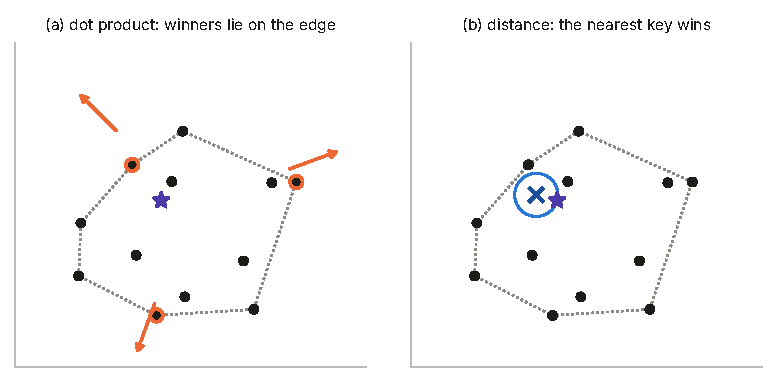
\includegraphics[width=0.75\textwidth]{figures/fig_cloud.pdf}
\caption{Which key can win, and why it matters for crowding. Black points are keys, the dotted line is the edge of the cloud, and the star is a key in the middle. (a) Dot product. For three query directions (arrows), the winning key is circled. It always lies on the edge. (b) Distance. A query (cross) near the star makes it the nearest key, so it wins. Appendix~\ref{app:geom} gives the details.}
\label{fig:cloud}
\end{figure}

We test the hypothesis in a small character-level language model.
Four design choices make the comparison fair.
The query and key projections are tied, so that the distance is a genuine metric.
The diagonal of the attention matrix is masked in every arm, because with tied projections a position is at distance zero from itself.
The scores of all arms are calibrated to the same spread at initialisation.
Every cell of the design has its own learning rate, chosen by a scan.

\Needspace{8\baselineskip}
The findings fall into three themes.
\begin{enumerate}
\item \textbf{The dot product scores better than the distance scores.} This holds in nearly every cell, and the difference is largest at the smallest head size, which is opposite to the hypothesis (Section~\ref{sec:dot}).
\item \textbf{The variation across exponents and head sizes is small.} To judge size, we include a control in which every allowed key receives the same weight, so that the model has no useful attention scores. This control is far worse than every other arm. Its gap to the best arm is about nine times the width of the band that contains all the dot-product and distance arms. The choice of score, exponent and head size therefore changes the result much less than having informative attention scores at all (Section~\ref{sec:flat}).
\item \textbf{The distance scores have costs.} They take several times longer to train in our implementation. They also learn faster early in training and fall behind later (Section~\ref{sec:cost}).
\end{enumerate}
\vspace{1em}

Section~\ref{sec:method} describes the design and Section~\ref{sec:results} the results.
Section~\ref{sec:discussion} offers labelled speculation and Section~\ref{sec:limits} states the limitations.
Section~\ref{sec:related} reviews related work.
The appendices give the mathematical background, the experimental details and the full results.

\section{Method}\label{sec:method}

We take a standard small decoder-only transformer language model and change one thing inside its self-attention blocks.
The changed element is the score that compares a query with a key.
The standard score is the dot product.
We replace it by minus an $\ell^p$ distance and compare the two rules at several head sizes $D$, where $D$ is the length of the query and key vectors.
A small $D$ leaves little room to separate many relationships, which is the crowding problem of the introduction.
The $\ell^p$ distance combines the differences of the coordinates of two vectors.
For $p=2$ it is the ordinary Euclidean distance, for $p=1$ it is the sum of the absolute differences, and for $p=\infty$ it is the largest single difference.
Everything else in the model is the same in all arms.

This section defines the scores, explains how their scales are matched, describes the model and the training, and states the statistical analysis.
Figure~\ref{fig:grid} at the end of the section summarises the design.

\subsection{Scores and arms}

Let $u_i$ be the normalised input of the attention block at position $i$, and let $s_{ij}$ be the score of query $i$ against key $j$ in one head.
The weights on the allowed keys $j$ are the softmax of the scores.
With tied projections the query and the key are both $z_i=Wu_i\in\mathbb{R}^D$.
The scores are
\begin{equation}
s_{ij}=\beta_h\,c\;z_i\!\cdot\! z_j\quad\text{(tied dot)},\qquad
s_{ij}=-\beta_h\,c\;d_p(z_i,z_j)\quad(\text{\Lp{} arms}),
\end{equation}
with
\begin{equation}
d_p(x,y)=\Big(\sum_{m=1}^{D}|x_m-y_m|^p+\varepsilon\Big)^{1/p}\ (p<\infty),\qquad d_\infty(x,y)=\max_m|x_m-y_m|.
\end{equation}
Here $\beta_h$ is a learned scale for each head, with initial value $1$ in every arm.
The constant $c$ is fixed after calibration (Section~\ref{sec:calib}).
It takes a different value in each arm, and also for each head size and layer.
The small number $\varepsilon$ keeps the gradient finite at exact matches.
It puts a floor under the distance of about 3 percent of the typical distance at $p=8$, and a smaller floor at smaller $p$ (Appendix~\ref{app:math}).

The arms are the tied dot product, which is the control, and seven $\ell^p$ distances with $p\in\{1,1.5,2,3,4,8,\infty\}$.
Two additional reference arms use separate query and key matrices.
The first is the untied dot product, which has one extra projection matrix per head.
The second is the untied dot product without the diagonal mask, run at $D=16$ only, which is the standard transformer.
A uniform control gives every allowed key the same weight.
It shows how much the attention scores can change the result.

As usual, query $i$ attends only to positions $j\le i$.
We also mask the diagonal $j=i$, except at position $0$, which has no other key.
The dot-product baseline is therefore slightly non-standard.
The unmasked reference measures the size of this departure.

\subsection{Calibration of the score scale}\label{sec:calib}

Different scores have different spreads across the keys, and the softmax is sensitive to the spread.
Each arm therefore multiplies its raw score by its own constant $c$, chosen at initialisation.
The constant is chosen so that the scores of a typical query have standard deviation about $1$ at initialisation.
It is measured separately for every arm, head size and layer, on fixed batches of text.
The target of $1$ was chosen by convention, and no other target was tried.
The learned scale $\beta_h$ was not tuned per arm.
Appendix~\ref{app:calib} gives the constants.

\subsection{Model, data and training}

The model is a decoder-only transformer \citep{radford2019} with pre-normalisation \citep{xiong2020}.
It has two layers, width $64$, four heads, an MLP of width $256$ and a context of $64$ characters.
Positions are learned absolute embeddings, and the input and output embeddings are tied \citep{press2017}.
Only the query-key dimension $D\in\{2,4,8,12,16\}$ varies, and the value width stays at $16$ per head.
The data are the Tiny Shakespeare text of \citet{karpathy2015}, which has about 1.1 million characters and 65 distinct symbols.
We split it 90/10 into training and validation text.
The outcome is the validation bits per character (bpc) after 4,000 training steps.
Appendix~\ref{app:setup} gives the optimiser and the schedule.

A seed fixes the data stream and the initial values of all shared parameters.
Arms run with the same seed therefore start from the same point and see the same batches, so their results are paired.
We use five seeds.
The design has 47 cells and 235 final runs, and no run diverged.

\subsection{Learning rates}

The best learning rate may depend on the arm and on $D$, so each cell has its own.
A one-seed scan over three rates chose the rate of each cell, with the scan seed outside the five final seeds.
Where the best rate lay at an end of the grid, one more rate was run beyond it.
The scan chose the same rate in all cells except the uniform control.
Per-arm tuning is therefore weak.
The rates were chosen on the validation set on which the results are reported.
Appendix~\ref{app:lr} gives the scan.

\subsection{Statistical analysis}

The five seeds serve as replicates.
For seed $s$, head size $D$ and exponent $p$, the paired gap to the tied dot product is
\begin{equation}
g_{s,D,p}=y_{s,D,p}-y_{s,D,\text{tied dot}},
\end{equation}
where $y$ is the final validation bpc.
A positive gap means that the $\ell^p$ arm is worse.
For each of the 35 cells we test the five seed gaps against zero with a one-sample $t$-test.
We report the mean gap with its 95\% interval, and a Holm-adjusted $p$-value \citep{holm1979} within each head size, over the seven arms.
To study how the gap changes with $D$, we fit for each seed and arm the least-squares slope of the gap on $\log_2 D$.
We test the five slopes against zero, for each arm and for their mean over the seven arms.
Two further contrasts are reported without correction.
They are untied minus tied dot at each $D$, and unmasked minus masked untied dot at $D=16$.
All other comparisons are descriptive.
Appendix~\ref{app:stats} gives the definitions.

Figure~\ref{fig:grid} shows the full design.
The crossed part has nine arms at five head sizes.
The uniform control and the unmasked untied dot product are two extra cells.
Every cell is run with five seeds, after a one-seed scan of the learning rate.

\begin{figure}[t]
\centering
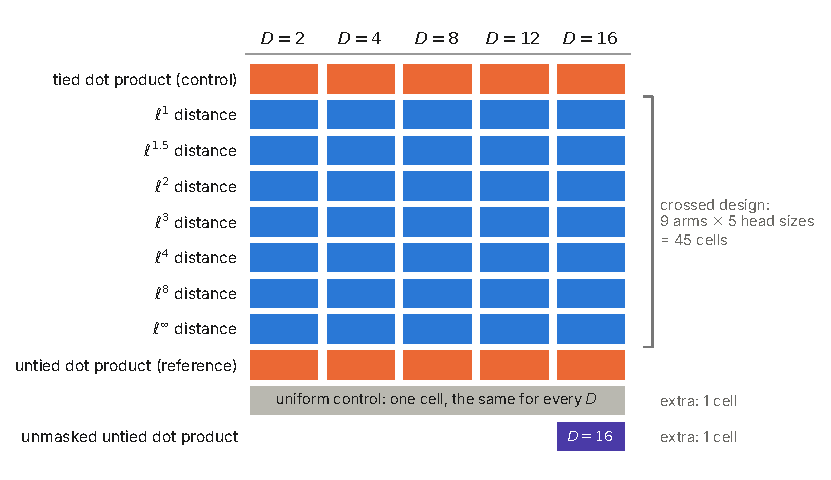
\includegraphics[width=0.9\textwidth]{figures/fig_grid.pdf}
\caption{The experimental design. Orange cells are dot-product arms and blue cells are $\ell^p$ arms. The nine arms at five head sizes form the crossed design with 45 cells. The uniform control and the unmasked untied dot product are two extra cells, which gives 47 cells in total.}
\label{fig:grid}
\end{figure}

\section{Results}\label{sec:results}

\subsection{Dot product versus distance scores}\label{sec:dot}

\begin{table}[t]
\centering\small
\begin{tabular}{rccccc}
\toprule
$D$ & Tied dot & Untied $-$ tied & Mean gap & Range of gaps & Gap $>0$ / significant (of 7) \\
\midrule
2 & 2.344 & -0.004 & +0.043 & $+0.036$ to $+0.050$ & 7 / 7 \\
4 & 2.340 & -0.007 & +0.017 & $+0.013$ to $+0.022$ & 7 / 3 \\
8 & 2.338 & -0.011 & +0.015 & $+0.008$ to $+0.024$ & 7 / 2 \\
12 & 2.334 & -0.005 & +0.020 & $+0.013$ to $+0.028$ & 7 / 2 \\
16 & 2.338 & -0.013 & +0.011 & $-0.005$ to $+0.026$ & 6 / 1 \\
\bottomrule
\end{tabular}

\caption{Results by head size $D$. Columns: mean validation bpc of the tied dot product; untied minus tied dot (bpc); mean over the seven $\ell^p$ arms of the gap to the tied dot (bpc); smallest and largest gap; number of the seven arms with a positive gap, and with a gap significant after Holm correction. A positive gap means that the $\ell^p$ arm is worse.}
\label{tab:summary}
\end{table}

\begin{figure}[t]
\centering
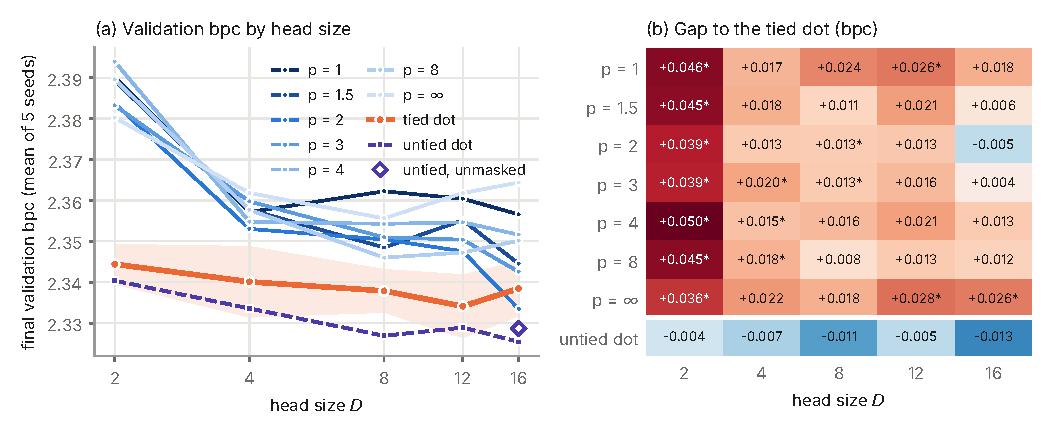
\includegraphics[width=\textwidth]{figures/fig_surface.pdf}
\caption{(a) Final validation bpc by head size, mean of five seeds. The shaded band is $\pm1$ seed standard deviation of the tied dot product. (b) Mean paired gap to the tied dot product. Red means that the arm is worse than the tied dot. An asterisk marks a cell that is significant after Holm correction within its head size ($p_{\text{Holm}}<0.05$). Full tables with the five single-seed gaps are in Appendix~\ref{app:full}.}
\label{fig:surface}
\end{figure}

\textbf{How the comparison is made.}
A cell is one arm at one head size.
Each cell has five final validation bpc values, one for each seed.
For each seed we subtract the bpc of the tied dot product, trained with the same seed and head size.
The difference is the gap of that seed.
A positive gap means that the $\ell^p$ arm has the higher bpc and is therefore worse.
Subtracting within a seed removes the variation that the two arms share, because runs with the same seed use the same data stream and the same starting point.

The five gaps of a cell differ from one another.
We ask whether their mean is far enough from zero to be distinguished from this variation.
The $t$ statistic is the mean gap divided by its standard error.
The standard error is the standard deviation of the five gaps divided by $\sqrt5$.
A large value of $|t|$ means that the mean lies many standard errors away from zero.
The $p$-value is the probability of a value of $|t|$ at least this large if the true mean gap were zero.
With five seeds we use the $t$ distribution with four degrees of freedom, which has heavier tails than the normal distribution and so asks for a larger $|t|$ at the same $p$.
The 95\% interval gives the values of the true mean gap that the data do not rule out.
We call a result significant when $p<0.05$.

We run seven such tests at each head size, one for each $\ell^p$ arm.
If all seven true gaps were zero and the tests were independent, the chance of at least one result with $p<0.05$ would be about 30 percent.
The Holm correction adjusts the seven $p$-values at each head size so that this chance stays below 5 percent.
A cell is called significant here only if its adjusted $p$-value is below $0.05$.
The correction makes the test conservative, so a cell that fails it may still have a real gap.
Table~\ref{tab:summary} counts, for each head size, the arms with a positive gap and the arms that pass the correction.

\textbf{Comparison across cells.}
The tied dot product has the lower bpc in \nPositive{} of the \nTested{} cells (Table~\ref{tab:summary}, Figure~\ref{fig:surface}).
The one exception is $p=2$ at $D=16$, where the gap is slightly negative and not significant.
After Holm correction, \nHolm{} of the \nTested{} cells are significant.
All seven cells at $D=2$ are among them.
At larger $D$ the gaps are smaller, and most single cells are not significant.
The evidence there rests mostly on the consistency of the sign across cells.
No cell favours an $\ell^p$ arm.

\textbf{Dependence on head size.}
The hypothesis predicts that the distance helps most at small $D$.
At small $D$ the gap would then be negative, and it would rise towards zero as $D$ grows.
We summarise the dependence on $D$ by a slope.
For each seed and each arm, we fit a straight line to the five gaps against $\log_2 D$.
The slope of this line is the change in the gap per doubling of the head size.
The hypothesis predicts a positive slope.
A negative slope means that the penalty of the distance shrinks as $D$ grows.

For the mean over the seven arms, we average the seven slopes within each seed.
This leaves five numbers, one for each seed.
We test whether their mean differs from zero, with the same $t$-test as above.
The observed slope is negative, and its interval excludes zero (Table~\ref{tab:tests}).
All five seed values are negative.
All seven arms also have a negative mean slope.
Five of them are individually significant at the 0.05 level, without correction, and the arms $p=1$ and $p=\infty$ are not (Appendix~\ref{app:full}).
The decline of the gap occurs mostly between $D=2$ and $D=4$ (Table~\ref{tab:summary}).
The data therefore point in the direction opposite to the hypothesis.

\begin{table}[t]
\centering\small
\begin{tabular}{lccc}
\toprule
Quantity (bpc) & Estimate & 95\% interval & $p$ \\
\midrule
Slope of the gap per doubling of $D$ (mean of seven arms) & -0.0086 & [-0.0127, -0.0044] & 0.0047 \\
Unmasked minus masked untied dot, $D=16$ & +0.003 & [-0.013, +0.020] & 0.61 \\
\bottomrule
\end{tabular}

\caption{Slope test and masking contrast. Both rows use a one-sample $t$-test on five seed values, without correction. Per-arm slopes are in Appendix~\ref{app:full}.}
\label{tab:tests}
\end{table}

\textbf{Untied dot product.}
The untied dot product has separate query and key matrices, so it has one more projection matrix than the tied dot product.
Comparing the two measures the cost of tying the query and key projections.
Untied minus tied dot is negative at all five head sizes (Table~\ref{tab:summary}).
This means that the untied arm is better.
We test each head size with the same $t$-test, without correction.
Only one head size gives a significant result, so the evidence at each head size is modest.
The sign is the same at every head size, which is consistent with a small benefit from untying.

\textbf{Masking.}
The unmasked untied dot product is the standard transformer, and it is run at $D=16$ only.
Comparing it with the masked untied dot product measures the effect of masking the diagonal.
We use the same $t$-test, without correction.
The two arms are not detectably different (Table~\ref{tab:tests}).
The interval is wide enough to include differences as large as many of the $\ell^p$ gaps.
We therefore claim that no cost of masking is detectable, and we do not claim that the cost is zero.

\subsection{Variation across exponents and head sizes}\label{sec:flat}

\begin{table}[t]
\centering\small
\begin{tabular}{lc}
\toprule
Quantity & bpc \\
\midrule
Lowest cell mean of the nine crossed arms & 2.325 \\
Highest cell mean of the nine crossed arms & 2.394 \\
Range & 0.068 \\
Uniform attention & 2.929 \\
Uniform attention minus highest crossed cell & 0.535 \\
Median seed standard deviation of a cell & 0.0096 \\
Tied dot, $D=2$ and $D=16$ & 2.344 and 2.338 \\
Largest spread of the seven $\ell^p$ arms within one $D$ ($D=16$) & 0.031 \\
Smallest such spread ($D=4$) & 0.009 \\
\bottomrule
\end{tabular}

\caption{Scale of the variation in final validation bpc.}
\label{tab:scale}
\end{table}

Table~\ref{tab:scale} gives the scale of the variation.
The nine arms at five head sizes occupy a narrow band.
That band is about a tenth as wide as the distance between the best of these arms and uniform attention.
Attention therefore has a large effect, and the choice among the crossed arms has a small one.
The spread between cells is a few times the seed standard deviation.
The tied dot product changes little between the smallest and the largest head.

The effect of $p$ is modest and shows no clear shape.
The spread of the seven $\ell^p$ arms within one head size is largest at $D=16$.
At $D=16$ the exponent $p=2$ is the best arm and $p=\infty$ the worst.
This dip is a single cell (Appendix~\ref{app:full}).
We report the variation across $p$ descriptively, without formal statistical tests.

\subsection{Costs and training dynamics}\label{sec:cost}

\textbf{Run time.}
Table~\ref{tab:time} gives the wall-clock time of one run.
The dot-product arms take about the same time at every $D$.
The $\ell^p$ arms take longer at every $D$, and their time grows with $D$.
The ratio to the tied dot product also grows with $D$.
These times come from four runs in parallel on a 2020 laptop.
They compare a chunked pure-PyTorch distance kernel \citep{paszke2019} with a matrix-multiplication dot product.
They do not describe the cost of the operations in general.

\begin{table}[t]
\centering\small
\begin{tabular}{lrrrrr}
\toprule
Arm & $D=2$ & $D=4$ & $D=8$ & $D=12$ & $D=16$ \\
\midrule
Tied dot & 7.7 & 7.7 & 7.9 & 7.2 & 8.5 \\
Untied dot & 7.2 & 7.6 & 7.9 & 8.2 & 8.2 \\
$p=1$ & 9.9 & 13.4 & 16.1 & 20.6 & 22.2 \\
$p=1.5$ & 14.5 & 19.3 & 27.6 & 35.2 & 41.6 \\
$p=2$ & 13.6 & 14.5 & 21.4 & 28.0 & 32.9 \\
$p=3$ & 13.2 & 16.8 & 24.3 & 33.5 & 38.1 \\
$p=4$ & 12.9 & 19.7 & 25.2 & 35.4 & 40.9 \\
$p=8$ & 14.3 & 19.0 & 33.4 & 42.0 & 49.1 \\
$p=\infty$ & 14.0 & 17.0 & 29.2 & 36.1 & 40.8 \\
\midrule
Fastest $\ell^p$ arm / tied dot & 1.3 & 1.7 & 2.0 & 2.9 & 2.6 \\
Slowest $\ell^p$ arm / tied dot & 1.9 & 2.6 & 4.2 & 5.8 & 5.8 \\
\midrule
Uniform attention (no scores) & \multicolumn{5}{c}{4.5} \\
\bottomrule
\end{tabular}

\caption{Mean wall-clock minutes per run (4,000 steps, five seeds), by arm and head size, and the ratio of the fastest and slowest $\ell^p$ arm to the tied dot product. Four runs in parallel, one thread each, on a 2020 Intel laptop.}
\label{tab:time}
\end{table}

\textbf{Early and late training.}
The $\ell^p$ arms are ahead of the tied dot product early in training.
At step 500 the $\ell^p$ arm has the lower validation bpc in almost all cells.
The mean gap changes sign near step 1,000, and the $\ell^p$ arms trail from then on (Figure~\ref{fig:training}; Appendix~\ref{app:training}).
We note this pattern without carrying out formal statistical tests.

\begin{figure}[t]
\centering
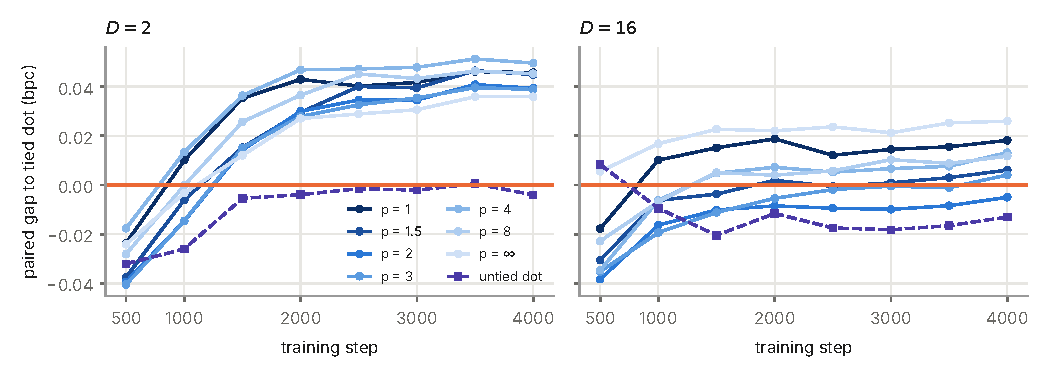
\includegraphics[width=\textwidth]{figures/fig_training.pdf}
\caption{Paired gap to the tied dot product during training at $D=2$ and $D=16$, mean of five seeds, evaluated every 500 steps. The orange line is the tied dot product. Above the line means worse. Appendix~\ref{app:training} shows all head sizes.}
\label{fig:training}
\end{figure}

\section{Discussion}\label{sec:discussion}

This section is speculative.
None of the explanations below was tested.
We state them because they bear on how the results should be read.

\paragraph{Why did the distance not help?}
We offer three candidates.
\begin{enumerate}
\item \textbf{The query-key space may not be crowded at this scale.} The tied dot product changes little between $D=16$ and $D=2$ (Table~\ref{tab:scale}). A two-dimensional head may already suffice for this task, so there may be little interference for a better score to remove. The crowding argument concerns separating many relationships in few dimensions. A character-level model with a context of 64 may rarely need to do this.
\item \textbf{The distance may be harder to optimise later in training.} The $\ell^p$ arms lead early and trail from about step 1,000. Their gradients are less regular than those of the dot product. They are sparse at $p=\infty$ and non-smooth at $p=1$. This does not explain $p=2$, which is smooth and still trails.
\item \textbf{The calibration matches the arms only at initialisation.} The dot product depends on the scale of the query vectors quadratically, and a distance depends on it linearly. The learned scale $\beta_h$ and the weights change during training, so the arms may drift apart. We logged the scales, the largest logits, the attention entropy and the query and key norms. We do not analyse them here.
\end{enumerate}

\paragraph{Why would the penalty shrink with $D$?}
At $D=2$ the head has two coordinates, and any non-Euclidean $\ell^p$ distance depends on the choice of axes (Appendix~\ref{app:math}).
A learned projection can choose its axes, but a two-dimensional projection has little room to do so.
We have no direct evidence for this explanation.
A second explanation is that the query-key space is least crowded at large $D$, so that less interference is left for a distance to remove (Appendix~\ref{app:super}).

\section{Limitations}\label{sec:limits}

\textbf{Sample size.}
Five seeds give wide intervals.
The smallest detectable paired difference is comparable to many of the gaps (Appendix~\ref{app:stats}).
Single cells at $D\ge4$ are mostly not individually significant.

\textbf{Scale.}
The model has two layers and width 64.
It trains for 4,000 steps on about 1.1 million characters.
Validation bpc changes by less than 0.01 on average over the last 500 steps, so the comparison is at an approximately converged budget but not at convergence.
Larger models, longer contexts and other data may behave differently.

\textbf{Learning rates.}
The learning-rate grid has steps of a factor of about 3, and almost every cell chose the same rate.
Differences between arms may therefore depend on how far each arm's own optimum lies from that rate.
We made no finer scan.
The rates were chosen on the validation set used for reporting.
The selection seed differs from the final seeds, and every arm was treated alike.

\textbf{Design choices.}
The score scale was not tuned per arm, and the target spread was chosen by convention.
The baseline is non-standard, because the diagonal is masked and the projections are tied.
The untied arm has one extra projection matrix.
Distances with $p\ne2$ depend on the coordinate axes.
The conclusions rest on learned absolute position embeddings.
The epsilon puts a floor under the distance, about 3 percent of the typical distance at $p=8$.

\textbf{Timing.}
The times describe our implementation on laptop CPUs.
A fused kernel or a GPU would change the ratios.

\textbf{Analysis.}
Tests of the effect of $p$ and of its interaction with $D$ are not reported.
The claim that no cost of masking is detectable is limited by the width of its interval.

\section{Related Work}\label{sec:related}

Several works replace the dot product by a distance for specific choices of metric.
\citet{kim2021lipschitz} show that dot-product attention is not Lipschitz, and that tying the query and key matrices makes the Euclidean version Lipschitz.
\citet{gulcehre2019hyperbolic} use a hyperbolic distance with a learned scale and offset.
\citet{mccarter2023inverse} derives inverse distance weighting from a distance score.
\citet{gao2025eco} use the $\ell^1$ distance to remove the matrix multiplications from attention.
\citet{williams2024stolen} describes a ``stolen attention'' effect in dot-product softmax, and reports that a negative squared Euclidean variant improves a question-answering benchmark.
We found no prior work that varies the exponent of an $\ell^p$ score across head sizes.

\citet{adler2026} studies how many token-token relations a single key-query channel can encode.
He shows that this number grows with the total key dimension, and that splitting a fixed total across several heads raises it.
The limit arises from interference between embeddings in superposition, a notion introduced for the features stored in network activations \citep{elhage2022}.
Our question is different: whether a different score function changes how a head of a given size copes with crowding.

Our tied dot product follows the Reformer, which shares queries and keys and masks the diagonal \citep{kitaev2020reformer}.
We use no query-key normalisation \citep{henry2020}, whose role in stabilising training is studied at scale by \citet{wortsman2024small}.
We use learned absolute positions, whereas rotary and relative position schemes \citep{shaw2018,su2021} change the form of the score and would interact with a distance.

\section{Conclusion and Future Work}

In a small character-level language model, an $\ell^p$ distance score did not beat the dot product at any head size.
The tied dot product was better in nearly every cell, and the penalty of the distance was largest at the smallest head size.
The conjecture that a distance relieves the crowding of a small query-key space was therefore not supported in this setting.
The untied dot product was better still, and masking the diagonal had no detectable cost.
All arms lay much closer to one another than to the control without informative attention scores.
The distance arms were also slower in our implementation.
They led early in training and fell behind later.

Several follow-up studies would test the explanations of Section~\ref{sec:discussion}.
\begin{itemize}
\item A finer learning-rate grid, or a sweep of the scale $\beta_h$, would test whether the penalty comes from tuning.
\item A task that requires singling out one key among many, such as the multi-query associative recall task of \citet{arora2024zoology}, would test the crowding argument directly, because it forces the query-key space to separate many relationships.
\item Learned relative position biases and longer contexts would test the dependence on absolute positions and on the number of keys.
\item An analysis of the logged scales, logits and norms would test the calibration explanation.
\end{itemize}

\section*{Acknowledgements}

Beyond the initial project design, this project's code, analysis and this write-up were developed in collaboration with Claude (Anthropic).

\begin{thebibliography}{99}
\setlength{\itemsep}{0.6em}
\bibitem[Adler(2026)]{adler2026}
Adler, M. (2026).
A capacity-based rationale for multi-head attention.
In \emph{Proceedings of the 43rd International Conference on Machine Learning}, volume 306 of \emph{Proceedings of Machine Learning Research}, pages 591--626.

\bibitem[Arora et al.(2024)]{arora2024zoology}
Arora, S., Eyuboglu, S., Timalsina, A., Johnson, I., Poli, M., Zou, J., Rudra, A., and R\'e, C. (2024).
Zoology: Measuring and improving recall in efficient language models.
In \emph{International Conference on Learning Representations}.

\bibitem[Ba et al.(2016)]{ba2016}
Ba, J. L., Kiros, J. R., and Hinton, G. E. (2016).
Layer normalization.
arXiv preprint arXiv:1607.06450.

\bibitem[Bhojanapalli et al.(2020)]{bhojanapalli2020}
Bhojanapalli, S., Yun, C., Rawat, A. S., Reddi, S., and Kumar, S. (2020).
Low-rank bottleneck in multi-head attention models.
In \emph{Proceedings of the 37th International Conference on Machine Learning}.

\bibitem[Elhage et al.(2022)]{elhage2022}
Elhage, N., Hume, T., Olsson, C., Schiefer, N., Henighan, T., Kravec, S., Hatfield-Dodds, Z., Lasenby, R., Drain, D., Chen, C., Grosse, R., McCandlish, S., Kaplan, J., Amodei, D., Wattenberg, M., and Olah, C. (2022).
Toy models of superposition.
arXiv preprint arXiv:2209.10652.

\bibitem[Gao et al.(2025)]{gao2025eco}
Gao, X., Amiraslani, S., Xu, X., and Xu, H. (2025).
EcoTransformer: Attention without multiplication.
arXiv preprint arXiv:2507.20096.

\bibitem[Gulcehre et al.(2019)]{gulcehre2019hyperbolic}
Gulcehre, C., Denil, M., Malinowski, M., Razavi, A., Pascanu, R., Hermann, K. M., Battaglia, P., Bapst, V., Raposo, D., Santoro, A., and de Freitas, N. (2019).
Hyperbolic attention networks.
In \emph{International Conference on Learning Representations}.

\bibitem[Hendrycks and Gimpel(2016)]{hendrycks2016}
Hendrycks, D. and Gimpel, K. (2016).
Gaussian error linear units (GELUs).
arXiv preprint arXiv:1606.08415.

\bibitem[Henry et al.(2020)]{henry2020}
Henry, A., Dachapally, P. R., Pawar, S., and Chen, Y. (2020).
Query-key normalization for transformers.
In \emph{Findings of the Association for Computational Linguistics: EMNLP 2020}.

\bibitem[Holm(1979)]{holm1979}
Holm, S. (1979).
A simple sequentially rejective multiple test procedure.
\emph{Scandinavian Journal of Statistics}, 6(2):65--70.

\bibitem[Karpathy(2015)]{karpathy2015}
Karpathy, A. (2015).
char-rnn.
\url{https://github.com/karpathy/char-rnn}.

\bibitem[Kim et al.(2021)]{kim2021lipschitz}
Kim, H., Papamakarios, G., and Mnih, A. (2021).
The Lipschitz constant of self-attention.
In \emph{Proceedings of the 38th International Conference on Machine Learning}.

\bibitem[Kitaev et al.(2020)]{kitaev2020reformer}
Kitaev, N., Kaiser, {\L}., and Levskaya, A. (2020).
Reformer: The efficient transformer.
In \emph{International Conference on Learning Representations}.

\bibitem[Loshchilov and Hutter(2017)]{loshchilov2017sgdr}
Loshchilov, I. and Hutter, F. (2017).
SGDR: Stochastic gradient descent with warm restarts.
In \emph{International Conference on Learning Representations}.

\bibitem[Loshchilov and Hutter(2019)]{loshchilov2019adamw}
Loshchilov, I. and Hutter, F. (2019).
Decoupled weight decay regularization.
In \emph{International Conference on Learning Representations}.

\bibitem[McCarter(2023)]{mccarter2023inverse}
McCarter, C. (2023).
Inverse distance weighting attention.
In \emph{NeurIPS 2023 Workshop on Associative Memory \& Hopfield Networks}.

\bibitem[Michel et al.(2019)]{michel2019}
Michel, P., Levy, O., and Neubig, G. (2019).
Are sixteen heads really better than one?
In \emph{Advances in Neural Information Processing Systems}, volume 32.

\bibitem[Pascanu et al.(2013)]{pascanu2013}
Pascanu, R., Mikolov, T., and Bengio, Y. (2013).
On the difficulty of training recurrent neural networks.
In \emph{Proceedings of the 30th International Conference on Machine Learning}.

\bibitem[Paszke et al.(2019)]{paszke2019}
Paszke, A., Gross, S., Massa, F., Lerer, A., Bradbury, J., Chanan, G., Killeen, T., Lin, Z., Gimelshein, N., Antiga, L., Desmaison, A., K\"opf, A., Yang, E., DeVito, Z., Raison, M., Tejani, A., Chilamkurthy, S., Steiner, B., Fang, L., Bai, J., and Chintala, S. (2019).
PyTorch: An imperative style, high-performance deep learning library.
In \emph{Advances in Neural Information Processing Systems}, volume 32.

\bibitem[Press and Wolf(2017)]{press2017}
Press, O. and Wolf, L. (2017).
Using the output embedding to improve language models.
In \emph{Proceedings of the 15th Conference of the European Chapter of the Association for Computational Linguistics}.

\bibitem[Radford et al.(2019)]{radford2019}
Radford, A., Wu, J., Child, R., Luan, D., Amodei, D., and Sutskever, I. (2019).
Language models are unsupervised multitask learners.
OpenAI technical report.

\bibitem[Shaw et al.(2018)]{shaw2018}
Shaw, P., Uszkoreit, J., and Vaswani, A. (2018).
Self-attention with relative position representations.
In \emph{Proceedings of the 2018 Conference of the North American Chapter of the Association for Computational Linguistics}.

\bibitem[Su et al.(2021)]{su2021}
Su, J., Lu, Y., Pan, S., Murtadha, A., Wen, B., and Liu, Y. (2021).
RoFormer: Enhanced transformer with rotary position embedding.
arXiv preprint arXiv:2104.09864.

\bibitem[Vaswani et al.(2017)]{vaswani2017}
Vaswani, A., Shazeer, N., Parmar, N., Uszkoreit, J., Jones, L., Gomez, A. N., Kaiser, L., and Polosukhin, I. (2017).
Attention is all you need.
In \emph{Advances in Neural Information Processing Systems}, volume 30.

\bibitem[Williams(2024)]{williams2024stolen}
Williams, K. (2024).
Stolen attention in transformers.
Technical Report NU-CS-2024-15, Northwestern University.

\bibitem[Wortsman et al.(2024)]{wortsman2024small}
Wortsman, M., Liu, P. J., Xiao, L., Everett, K., Alemi, A., Adlam, B., Co-Reyes, J. D., Gur, I., Kumar, A., Novak, R., Pennington, J., Sohl-Dickstein, J., Xu, K., Lee, J., Gilmer, J., and Kornblith, S. (2024).
Small-scale proxies for large-scale Transformer training instabilities.
In \emph{International Conference on Learning Representations}.

\bibitem[Xiong et al.(2020)]{xiong2020}
Xiong, R., Yang, Y., He, D., Zheng, K., Zheng, S., Xing, C., Zhang, H., Lan, Y., Wang, L., and Liu, T.-Y. (2020).
On layer normalization in the Transformer architecture.
In \emph{Proceedings of the 37th International Conference on Machine Learning}.
\end{thebibliography}

\appendix

\section{Mathematical background}\label{app:math}

\subsection{Geometry of the scores}\label{app:geom}

This section explains why a dot product and a distance pick out keys differently.
We work with one query $q\in\mathbb{R}^D$ and a finite set of keys $k_1,\dots,k_n\in\mathbb{R}^D$.
These stand for the projected vectors of the earlier positions.
The softmax gives more weight to a key with a higher score.
We say that a key \emph{wins} if its score is strictly higher than that of every other key.
The questions below ask which keys can win.
They do not claim that a trained model needs to single out particular keys.

\paragraph{Level sets.}
A score assigns a number to every point $k$.
The \emph{level set} of a score is the set of points with the same score.
Figure~\ref{fig:levelsets} shows the level sets for $D=2$.

\begin{figure}[h]
\centering
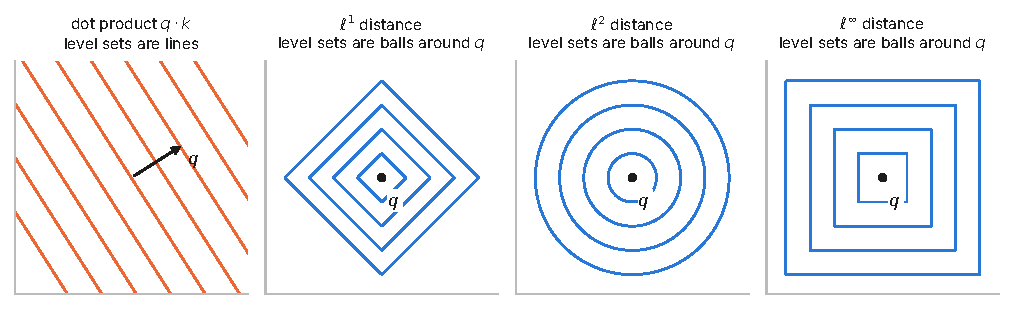
\includegraphics[width=\textwidth]{figures/fig_levelsets.pdf}
\caption{Level sets of the score of one query $q$ in two dimensions. Each curve joins the points $k$ that receive the same score. For the dot product the curves are parallel lines and the score grows in the direction of $q$. For a distance the curves are balls around $q$, and the score grows towards $q$.}
\label{fig:levelsets}
\end{figure}

\paragraph{The dot product.}
The score is $s(k)=q\cdot k$.
The level set $\{k: q\cdot k=\tau\}$ is a line when $D=2$, and a hyperplane in general.
It is perpendicular to $q$.
As $\tau$ grows, the line moves in the direction of $q$.
The winner is therefore the key $k_m$ with the largest value of $q\cdot k_m$, which is the key that lies furthest in the direction of $q$.

\begin{proposition}\label{prop:edge}
Suppose that $k_m$ can be written as a weighted average of the other keys, $k_m=\sum_{j\ne m}\lambda_j k_j$ with $\lambda_j\ge0$ and $\sum_{j\ne m}\lambda_j=1$.
Then for every query $q$ we have $q\cdot k_m\le\max_{j\ne m}q\cdot k_j$, so $k_m$ never wins.
\end{proposition}
\begin{proof}
By linearity, $q\cdot k_m=\sum_{j\ne m}\lambda_j\,(q\cdot k_j)$.
A weighted average of numbers cannot exceed their maximum.
\end{proof}

The keys that are not weighted averages of the others are the corners of the convex hull of the keys.
Here the convex hull is the smallest convex region that contains all the keys, like a rubber band stretched around them.
The proposition says that only these corner keys can win under a dot product.
Figure~\ref{fig:interior}(a) shows this.
For each of three directions $q$, the dashed line is the level set through the winning key.
All other keys lie on the lower-scoring side of that line, so the winner is a corner of the hull.
The key marked by a star is inside the hull, and it does not win for any $q$.

\paragraph{The distance.}
The score is $s(k)=-d_p(q,k)$.
The level set $\{k: d_p(q,k)=r\}$ is the $\ell^p$ ball of radius $r$ around $q$.
In two dimensions it is the set $|x_1|^p+|x_2|^p=r^p$ with $x=k-q$.
It is a diamond for $p=1$, a circle for $p=2$ and a square for $p=\infty$ (Figure~\ref{fig:levelsets}).
The score grows as $k$ approaches $q$, so the winner is the key nearest to $q$.

\begin{proposition}\label{prop:nearest}
Let $k_m$ be any key that differs from all the others, and take $q=k_m$.
Then $d_p(q,k_m)=0<d_p(q,k_j)$ for every $j\ne m$, so $k_m$ wins.
The same holds for every $q$ close enough to $k_m$.
\end{proposition}
\begin{proof}
The distance is zero only between identical points, so $d_p(k_m,k_j)>0$ for all $j\ne m$.
The distance is continuous in $q$, so these inequalities persist in a neighbourhood of $k_m$.
\end{proof}

Figure~\ref{fig:interior}(b) shows this.
A query placed near the starred key makes it the nearest key, and the circle around the query contains no other key.
Under a distance, a key in the middle of the cloud can therefore win.

\begin{figure}[h]
\centering
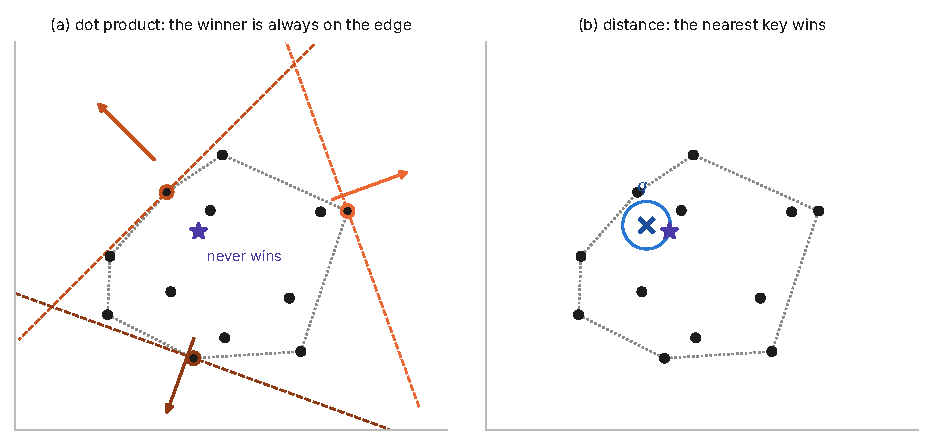
\includegraphics[width=0.9\textwidth]{figures/fig_interior.pdf}
\caption{Which keys can win. The black points are keys, the dotted line is the boundary of their convex hull, and the star is a key inside the hull. (a) Dot product. For each of three query directions (arrows), the dashed line is the level set through the winning key, circled. The winner is always a corner of the hull. (b) Distance. A query (cross) placed near the starred key makes it the nearest key, and the circle through that key contains no other key.}
\label{fig:interior}
\end{figure}

\paragraph{Limits of the argument.}
The argument concerns which key can have the highest score.
Under a dot product, an interior key still receives some softmax weight.
The model also learns the queries and the keys, so it can place the keys where it needs them.
The argument therefore motivates the question, and it does not predict that a distance performs better.
Appendix~\ref{app:super} connects it to crowding.
A dot product with a key-dependent bias does not have the restriction.
Appendix~\ref{app:sq} shows that squared Euclidean distance is such a score.

\subsection{Crowding: why small heads may be limited}\label{app:super}

This section gives two heuristic arguments for the conjecture of the introduction.
Both compare how well a dot product and a distance separate many keys in few dimensions.
Neither is a theorem about trained models.

\paragraph{Setting.}
Crowding arises when a space must separate more items than it has well-spaced places.
The problem resembles superposition, where features share directions and interfere \citep{elhage2022}, but we use no result from that literature.
In an attention head, the items are the keys that a query must tell apart.
A query selects a key if that key has the highest score and the gap to the other keys is large enough for the softmax to concentrate on it.
When $D$ is small there are few well-separated places to put keys, so many keys must lie close together.

\paragraph{Margins on a circle.}
Take $D=2$ and let $P$ keys be equally spaced unit vectors on a circle.
Let the query equal one of the keys, so that this key is the correct target.
The nearest rival lies at an angle $2\pi/P$ from the target.
The dot-product scores of the target and of the rival are $1$ and $\cos(2\pi/P)$.
Their gap is
\begin{equation}
1-\cos(2\pi/P)\approx\frac{2\pi^2}{P^2}.
\end{equation}
The scores of the distance are $0$ and $-2\sin(\pi/P)$.
Their gap is
\begin{equation}
2\sin(\pi/P)\approx\frac{2\pi}{P}.
\end{equation}
The dot-product gap shrinks like $P^{-2}$ because the cosine is flat at its peak.
The distance gap shrinks like $P^{-1}$ because the distance changes linearly near a match.
The calibration of Section~\ref{sec:calib} fixes the spread of the scores over keys, so the relevant quantity is the gap divided by that spread.
Table~\ref{tab:margin} gives this quantity.
To give the target a fixed logit lead over its nearest rival, the dot product needs a scale larger by the ratio in the last column.
The ratio grows in proportion to $P$.

\begin{table}[h]
\centering\small
\begin{tabular}{rccc}
\toprule
$P$ & Dot product & Distance & Ratio \\
\midrule
16 & 0.1077 & 0.625 & 5.8 \\
32 & 0.0272 & 0.317 & 11.7 \\
64 & 0.0068 & 0.159 & 23.4 \\
128 & 0.0017 & 0.080 & 46.8 \\
\bottomrule
\end{tabular}

\caption{Score gap between a key and its nearest rival, divided by the standard deviation of the scores over all keys, for $P$ equally spaced unit vectors on a circle. The last column is the ratio of the distance value to the dot-product value.}
\label{tab:margin}
\end{table}

\paragraph{Counting winnable keys.}
By Proposition~\ref{prop:edge}, only keys on the edge of the key cloud can win under a dot product.
Suppose the keys lie in a ball.
Keys that must be told apart by at least a separation $\epsilon$ can then occupy the $(D-1)$-dimensional surface under a dot product, and the $D$-dimensional volume under a distance.
The numbers of such keys scale like $\epsilon^{-(D-1)}$ and $\epsilon^{-D}$.
For $P$ keys, the separation that can be achieved scales like $P^{-1/(D-1)}$ for the dot product and $P^{-1/D}$ for the distance.
The gap between these two exponents is large at $D=2$ and small at $D=16$.
Table~\ref{tab:pack} checks this by a greedy random packing.
The ratio of the two counts grows as the separation shrinks, and it is smaller at larger $D$.
The counts come from one random sequence each.
Ratios below one at coarse separation are sampling noise.

\begin{table}[h]
\centering\small
\begin{tabular}{rcccc}
\toprule
$D$ & Separation & Keys on the sphere & Keys in the ball & Ratio \\
\midrule
2 & 0.5 & 10 & 12 & 1.20 \\
2 & 0.35 & 14 & 21 & 1.50 \\
2 & 0.25 & 19 & 40 & 2.11 \\
\addlinespace
3 & 0.5 & 33 & 31 & 0.94 \\
3 & 0.35 & 65 & 81 & 1.25 \\
3 & 0.25 & 126 & 193 & 1.53 \\
\addlinespace
4 & 0.5 & 94 & 85 & 0.90 \\
4 & 0.35 & 257 & 252 & 0.98 \\
4 & 0.25 & 615 & 721 & 1.17 \\
\bottomrule
\end{tabular}

\caption{Greedy random packing of points with mutual distance at least the separation, on the unit sphere and in the unit ball. The ratio is the count in the ball divided by the count on the sphere.}
\label{tab:pack}
\end{table}

\paragraph{Qualifications.}
For keys and queries of equal norm, squared Euclidean distance and the dot product give the same ranking, because $\|q-k\|^2=2-2\,q\cdot k$.
A distance therefore differs from a dot product through the variation of the norms, or through the shape of the score.
A learned scale can partly compensate for the flat peak of the dot product, at the cost of a larger logit range.
In high dimensions a dot product can also use many nearly orthogonal directions, so it is not intrinsically poor at separating many keys.
We therefore state the conjecture for small $D$ only.

\subsection{Coincidences between exponents}

At $D=1$ all $\ell^p$ distances equal $|x-y|$.
At $D=2$ the following relation holds.

\begin{proposition}\label{prop:two}
Let $A=\begin{pmatrix}1&1\\1&-1\end{pmatrix}$. For all $x,y\in\mathbb{R}^2$, $d_1(x,y)=d_\infty(Ax,Ay)$.
\end{proposition}
\begin{proof}
Write $a=x_1-y_1$ and $b=x_2-y_2$.
Then $A(x-y)=(a+b,\,a-b)$, so $d_\infty(Ax,Ay)=\max(|a+b|,|a-b|)$.
Now $(a+b)^2$ and $(a-b)^2$ differ by $4ab$, so the larger of the two is $a^2+b^2+2|ab|=(|a|+|b|)^2$.
Hence $\max(|a+b|,|a-b|)=|a|+|b|=d_1(x,y)$.
\end{proof}

With tied projections $z=Wu$, an $\ell^1$ model with projection $W$ and an $\ell^\infty$ model with projection $AW$ give the same distances.
At $D=2$ the two arms therefore have equal expressive power, and any difference between them reflects optimisation.

\subsection{Gradient and the epsilon floor}

For finite $p>1$ the gradient of $d_p$ with respect to $x$ is
\begin{equation}
\frac{\partial d_p}{\partial x_m}=\operatorname{sign}(x_m-y_m)\,|x_m-y_m|^{p-1}\,d_p^{\,1-p}.
\end{equation}
At $x=y$ the factor $d_p^{1-p}$ is infinite, so $\varepsilon$ is added inside the root.
We set $\varepsilon=r\,S_{\mathrm{typ}}$, where $S_{\mathrm{typ}}$ is the median of $\sum_m|x_m-y_m|^p$ over the calibration pairs, measured at initialisation and then frozen, and $r=10^{-12}$.
At an exact match the distance equals $\varepsilon^{1/p}=r^{1/p}S_{\mathrm{typ}}^{1/p}$.
This is the fraction $r^{1/p}$ of the typical distance.
The fraction is $10^{-1.5}\approx3\%$ at $p=8$, $0.1\%$ at $p=4$, $0.01\%$ at $p=3$, $10^{-6}$ at $p=2$ and $10^{-8}$ at $p=1.5$.
No epsilon is needed at $p=1$.
For $p=\infty$ the distance is a maximum, the gradient goes to the coordinates that attain it, and it is split evenly among ties.
All distances are computed in 32-bit floating point.
The $p=2$ distance is computed from coordinate differences like all others, and not from the expansion $\|x-y\|^2=\|x\|^2+\|y\|^2-2x\cdot y$, which loses accuracy for nearby vectors.

\subsection{Squared Euclidean distance and the dot product}\label{app:sq}

For a fixed query, $-\tfrac12\|q-k\|^2=q\cdot k-\tfrac12\|k\|^2-\tfrac12\|q\|^2$.
The last term does not depend on the key, so it cancels in the softmax over keys.
Squared Euclidean attention therefore equals dot-product attention with a key-dependent bias $-\tfrac12\|k\|^2$.
The plain Euclidean distance has no such reduction, so the tied dot product and the $\ell^2$ arm are different controls.

\subsection{Why the scale needs calibration}

Suppose the coordinates of $z_i-z_j$ are independent with scale $\sigma$.
Then $S=\sum_m|z_{i,m}-z_{j,m}|^p$ has mean proportional to $D$ and variance proportional to $D$.
The delta method for $d=S^{1/p}$ gives
\begin{equation}
\operatorname{sd}(d_p)\;\propto\;\sigma\,D^{1/p-1/2}.
\end{equation}
The spread of the distance across keys therefore depends on $p$ and on $D$ in a different way for each exponent.
For $p=2$ the exponent is zero.
The argument fails at $p=\infty$.
The dot product of the same vectors has spread proportional to $\sqrt{D}$, which motivates the usual factor $1/\sqrt{D}$.
Real activations have correlated coordinates, so we do not use the formula.
We measure $c$ on real batches (Appendix~\ref{app:calib}).

\section{Experimental details}\label{app:setup}

\subsection{Model, data and training}

\begin{itemize}
\item \textbf{Data.} Tiny Shakespeare \citep{karpathy2015}, 1,115,394 characters, md5 \texttt{6fb458f1232090904f\allowbreak b40fe944165e91}. The split is 90/10. Validation uses the whole validation text in non-overlapping windows of 64.
\item \textbf{Model.} Decoder-only, pre-norm \citep{ba2016}, two layers, width 64, four heads, MLP width 256 with GELU \citep{hendrycks2016}, context 64, learned absolute positions, tied input and output embeddings. The query, key and value projections have no bias. The tied matrix is stored once, and the untied arm starts with the same matrix as the tied arms.
\item \textbf{Initialisation.} Projections start with standard deviation $0.02$. The coordinates of $z$ then have a standard deviation of about $0.16$, so the constant of the tied dot product is near $40/\sqrt D$ and not near $1/\sqrt D$.
\item \textbf{Optimiser.} AdamW \citep{loshchilov2019adamw} with $\beta=(0.9,0.95)$, weight decay $0.01$ on the weight matrices only, and gradient clipping \citep{pascanu2013} at global norm $1.0$.
\item \textbf{Schedule.} Batch of 64 sequences of 64 characters, 4,000 steps. Linear warm-up over 200 steps, then cosine decay \citep{loshchilov2017sgdr} to $10\%$ of the peak rate.
\item \textbf{Evaluation.} Every 500 steps and at the end. The outcome is the value at step 4,000, not the best value during training.
\item \textbf{Divergence.} A run counts as diverged if its training loss is non-finite or its final validation bpc exceeds $\log_2 65\approx6.02$. No run met this condition.
\item \textbf{Logging.} Each run logs the learned scales, the largest logit, the attention entropy and the query and key norms at every evaluation.
\end{itemize}

\subsection{Cells and runs}

The crossed design has nine arms at five head sizes, which gives 45 cells.
The uniform control (one cell) and the unmasked untied dot product at $D=16$ (one cell) bring the total to 47.
Each cell has five final seeds ($1$ to $5$), so there are 235 main runs.
The learning-rate scan used seed 100.
It has $47\times3=141$ base runs and 46 extra runs at $10^{-3}$, which makes 187 runs.
No run diverged.

\subsection{Compute}

Runs used PyTorch \citep{paszke2019} on a 2020 Intel MacBook, with four worker processes of one thread each.
The main runs took \totalHoursMain{} hours of summed wall-clock time.
Six scan runs and nine main runs were resumed from a checkpoint after an interruption.

\subsection{Integrity checks}

Before the analysis we checked the following.
\begin{itemize}
\item All 235 main and 187 scan runs are present with all their files, the same five seeds appear in every cell, and no value is missing.
\item The final validation bpc in each \texttt{result.json} equals the last row of its \texttt{log.csv}, and the learning-rate column follows the schedule.
\item Each main run used the rate in the selection file, and each selected rate is the lowest-bpc rate of its scan.
\item All 235 stored final weights reload and reproduce the stored validation bpc to about $10^{-7}$.
\item The stored calibration constants and epsilons match the calibration files in all 828 layers of the scan and main runs.
\item The nine resumed main runs are not outliers within their cells (largest deviation 1.5 seed standard deviations).
\item Rerunning the analysis stage reproduces all tables exactly, and an independent recomputation of the tables used here agrees with them up to the six-digit rounding of the files.
\end{itemize}

\section{Calibration constants}\label{app:calib}

The constant $c$ is the inverse of the root mean square of the per-query standard deviations of the raw scores.
The pooling uses 32 fixed batches of 64 sequences, the allowed keys of positions with at least 8 allowed keys, and the four heads of the layer.
The model is built with a fixed calibration seed, and all seeds share the result.
The unmasked arm is calibrated over all its allowed keys, including the position itself.

\begin{table}[h]
\centering\small
\begin{tabular}{lrrrrr}
\toprule
Arm & $D=2$ & $D=4$ & $D=8$ & $D=12$ & $D=16$ \\
\midrule
Tied dot & 27.18 / 28.95 & 19.72 / 19.74 & 12.49 / 14.16 & 10.15 / 10.80 & 8.35 / 8.92 \\
Untied dot & 26.32 / 28.77 & 19.94 / 20.93 & 14.07 / 15.48 & 11.83 / 12.87 & 10.33 / 11.26 \\
Untied dot, unmasked & -- & -- & -- & -- & 10.35 / 11.19 \\
$p=1$ & 6.22 / 6.13 & 4.31 / 4.14 & 2.80 / 2.94 & 2.26 / 2.30 & 1.88 / 1.96 \\
$p=1.5$ & 7.49 / 7.49 & 6.47 / 6.30 & 5.24 / 5.53 & 4.82 / 4.91 & 4.42 / 4.58 \\
$p=2$ & 8.02 / 8.11 & 7.63 / 7.53 & 6.87 / 7.30 & 6.73 / 6.86 & 6.47 / 6.70 \\
$p=3$ & 8.39 / 8.59 & 8.57 / 8.61 & 8.38 / 8.99 & 8.67 / 8.92 & 8.72 / 9.04 \\
$p=4$ & 8.49 / 8.75 & 8.85 / 8.99 & 8.87 / 9.57 & 9.31 / 9.66 & 9.53 / 9.91 \\
$p=8$ & 8.56 / 8.87 & 8.99 / 9.24 & 9.06 / 9.84 & 9.50 / 9.98 & 9.79 / 10.24 \\
$p=\infty$ & 8.56 / 8.89 & 8.96 / 9.25 & 8.93 / 9.71 & 9.25 / 9.77 & 9.46 / 9.93 \\
\bottomrule
\end{tabular}

\caption{Calibration constant $c$ of layer 1 / layer 2, by arm and head size.}
\end{table}

For the tied dot product the coordinates of $z$ have variance $\sigma_z^2$, and the constant should satisfy $c\,\sigma_z^2\sqrt D\approx1$.
Table~\ref{tab:calibcheck} shows that it does, to within 16 percent.

\begin{table}[h]
\centering\small
\begin{tabular}{lrrrrr}
\toprule
Layer & $D=2$ & $D=4$ & $D=8$ & $D=12$ & $D=16$ \\
\midrule
1 & 1.02 & 0.97 & 0.92 & 0.88 & 0.84 \\
2 & 1.00 & 0.95 & 0.94 & 0.88 & 0.84 \\
\bottomrule
\end{tabular}

\caption{The check $c\,\sigma_z^2\sqrt D$ for the tied dot product, by layer and head size.}
\label{tab:calibcheck}
\end{table}

\section{Learning-rate scan}\label{app:lr}

Table~\ref{tab:scan} gives the validation bpc of the scan run at each rate.
The chosen rate is in bold.
The rate $3\cdot10^{-3}$ beat $10^{-3}$ by a median of \marginOverThousandMedian{} bpc and beat $10^{-2}$ by a median of \marginOverTenMedian{} bpc.
No cell needed the extra rate $9\cdot10^{-2}$.
The scan seed is outside the final seeds, and scan runs are not pooled with the main results.

{\small
\begin{longtable}{llrrrrr}
\toprule
Arm & $D$ & $10^{-3}$ & $3\cdot10^{-3}$ & $10^{-2}$ & $3\cdot10^{-2}$ & Chosen \\
\midrule
\endhead
Tied dot & 2 & 2.490 & \textbf{2.357} & 2.366 & 2.435 & 0.003 \\
Tied dot & 4 & 2.467 & \textbf{2.340} & 2.376 & 2.441 & 0.003 \\
Tied dot & 8 & 2.448 & \textbf{2.345} & 2.371 & 2.453 & 0.003 \\
Tied dot & 12 & 2.436 & \textbf{2.323} & 2.380 & 2.457 & 0.003 \\
Tied dot & 16 & 2.433 & \textbf{2.331} & 2.345 & 2.483 & 0.003 \\
Untied dot & 2 & 2.472 & \textbf{2.339} & 2.344 & 2.413 & 0.003 \\
Untied dot & 4 & 2.466 & \textbf{2.325} & 2.350 & 2.406 & 0.003 \\
Untied dot & 8 & 2.429 & \textbf{2.336} & 2.366 & 2.429 & 0.003 \\
Untied dot & 12 & 2.423 & \textbf{2.319} & 2.362 & 2.421 & 0.003 \\
Untied dot & 16 & 2.428 & \textbf{2.333} & 2.343 & 2.431 & 0.003 \\
Untied dot, unmasked & 16 & 2.440 & \textbf{2.346} & 2.366 & 2.462 & 0.003 \\
$p=1$ & 2 & 2.479 & \textbf{2.386} & 2.389 & 2.459 & 0.003 \\
$p=1$ & 4 & 2.465 & \textbf{2.371} & 2.384 & 2.430 & 0.003 \\
$p=1$ & 8 & 2.444 & \textbf{2.354} & 2.407 & 2.448 & 0.003 \\
$p=1$ & 12 & 2.432 & \textbf{2.365} & 2.400 & 2.439 & 0.003 \\
$p=1$ & 16 & 2.443 & \textbf{2.346} & 2.386 & 2.446 & 0.003 \\
$p=1.5$ & 2 & 2.474 & \textbf{2.367} & 2.411 & 2.436 & 0.003 \\
$p=1.5$ & 4 & 2.451 & \textbf{2.364} & 2.393 & 2.425 & 0.003 \\
$p=1.5$ & 8 & 2.428 & \textbf{2.345} & 2.380 & 2.438 & 0.003 \\
$p=1.5$ & 12 & 2.430 & \textbf{2.355} & 2.375 & 2.432 & 0.003 \\
$p=1.5$ & 16 & 2.425 & \textbf{2.338} & 2.389 & 2.430 & 0.003 \\
$p=2$ & 2 & 2.473 & \textbf{2.391} & 2.398 & 2.464 & 0.003 \\
$p=2$ & 4 & 2.446 & \textbf{2.364} & 2.409 & 2.451 & 0.003 \\
$p=2$ & 8 & 2.411 & \textbf{2.331} & 2.410 & 2.419 & 0.003 \\
$p=2$ & 12 & 2.420 & \textbf{2.317} & 2.404 & 2.429 & 0.003 \\
$p=2$ & 16 & 2.404 & \textbf{2.341} & 2.379 & 2.414 & 0.003 \\
$p=3$ & 2 & 2.463 & \textbf{2.357} & 2.418 & 2.474 & 0.003 \\
$p=3$ & 4 & 2.457 & \textbf{2.358} & 2.404 & 2.436 & 0.003 \\
$p=3$ & 8 & 2.420 & \textbf{2.332} & 2.391 & 2.438 & 0.003 \\
$p=3$ & 12 & 2.408 & \textbf{2.327} & 2.380 & 2.421 & 0.003 \\
$p=3$ & 16 & 2.424 & \textbf{2.354} & 2.407 & 2.435 & 0.003 \\
$p=4$ & 2 & 2.444 & \textbf{2.371} & 2.399 & 2.448 & 0.003 \\
$p=4$ & 4 & 2.448 & \textbf{2.374} & 2.400 & 2.433 & 0.003 \\
$p=4$ & 8 & 2.435 & \textbf{2.342} & 2.390 & 2.426 & 0.003 \\
$p=4$ & 12 & 2.422 & \textbf{2.342} & 2.377 & 2.452 & 0.003 \\
$p=4$ & 16 & 2.419 & \textbf{2.342} & 2.401 & 2.442 & 0.003 \\
$p=8$ & 2 & 2.456 & \textbf{2.356} & 2.387 & 2.432 & 0.003 \\
$p=8$ & 4 & 2.458 & \textbf{2.364} & 2.390 & 2.429 & 0.003 \\
$p=8$ & 8 & 2.432 & \textbf{2.353} & 2.382 & 2.455 & 0.003 \\
$p=8$ & 12 & 2.419 & \textbf{2.350} & 2.407 & 2.431 & 0.003 \\
$p=8$ & 16 & 2.426 & \textbf{2.351} & 2.397 & 2.432 & 0.003 \\
$p=\infty$ & 2 & 2.470 & \textbf{2.392} & 2.406 & 2.482 & 0.003 \\
$p=\infty$ & 4 & 2.461 & \textbf{2.369} & 2.406 & 2.459 & 0.003 \\
$p=\infty$ & 8 & 2.439 & \textbf{2.339} & 2.397 & 2.415 & 0.003 \\
$p=\infty$ & 12 & 2.452 & \textbf{2.354} & 2.380 & 2.417 & 0.003 \\
$p=\infty$ & 16 & 2.427 & \textbf{2.349} & 2.393 & 2.407 & 0.003 \\
Uniform attention & -- & -- & 2.986 & \textbf{2.906} & 2.948 & 0.01 \\
\bottomrule
\end{longtable}

}
\begingroup\captionof{table}{Validation bpc of the one-seed scan (seed 100). Bold marks the chosen rate. A dash means that the rate was not run.}\label{tab:scan}\endgroup

\section{Statistical definitions}\label{app:stats}

\textbf{Cell gaps.}
For a cell $(D,p)$ let $\bar g$ and $s$ be the mean and standard deviation of the five seed gaps $g_{1,D,p},\dots,g_{5,D,p}$.
The statistic is $t=\bar g/(s/\sqrt5)$ with 4 degrees of freedom.
The 95\% interval is $\bar g\pm t_{0.975,4}\,s/\sqrt5$ with $t_{0.975,4}=2.776$.
The variation between seeds is contained in $s$.
The pairing removes what the arms of one seed share, which is the data stream and the initial parameters.

\textbf{Holm correction.}
Within a head size, sort the seven $p$-values as $p_{(1)}\le\dots\le p_{(7)}$.
The adjusted values are $\tilde p_{(k)}=\min\{1,\max_{j\le k}(8-j)\,p_{(j)}\}$.
The families of different head sizes are not combined.

\textbf{Trend.}
For seed $s$ and arm $p$ let $\hat\beta_{s,p}$ be the least-squares slope of $g_{s,D,p}$ on $\log_2 D$ over the five head sizes.
The slope is in bpc per doubling of $D$.
The mean row averages the seven arms within each seed first.
Each row is tested with a one-sample $t$-test on five values.
No correction is applied across the eight rows.

\textbf{Assumptions.}
The $t$-tests assume that the five values are approximately normal.
With five seeds, the exact sign test and the signed-rank test cannot give a two-sided $p$-value below $2/2^5=0.0625$, so the $t$-test is the only simple option.

\textbf{Detectable differences.}
The median standard deviation of a paired seed gap is 0.012 bpc.
A Monte Carlo power calculation for the paired $t$-test with five seeds gives a smallest detectable difference of 1.69 standard deviations at the 0.05 level, and 2.88 standard deviations at the level 0.05/7 used for seven arms, both at 80 percent power.
These correspond to about 0.021 bpc and 0.035 bpc.

\textbf{Uncorrected contrasts.}
The untied minus tied dot gaps at each head size and the unmasked minus masked gap at $D=16$ are tested in the same way, without correction.

\section{Full results}\label{app:full}

\begin{table}[h]
\centering\small
\begin{tabular}{lccccc}
\toprule
Arm & $D=2$ & $D=4$ & $D=8$ & $D=12$ & $D=16$ \\
\midrule
Tied dot & 2.344 $\pm$ 0.005 & 2.340 $\pm$ 0.009 & 2.338 $\pm$ 0.005 & 2.334 $\pm$ 0.008 & 2.338 $\pm$ 0.007 \\
Untied dot & 2.340 $\pm$ 0.012 & 2.334 $\pm$ 0.010 & 2.327 $\pm$ 0.006 & 2.329 $\pm$ 0.006 & 2.325 $\pm$ 0.009 \\
$p=1$ & 2.390 $\pm$ 0.027 & 2.357 $\pm$ 0.015 & 2.362 $\pm$ 0.015 & 2.360 $\pm$ 0.007 & 2.357 $\pm$ 0.008 \\
$p=1.5$ & 2.389 $\pm$ 0.015 & 2.358 $\pm$ 0.003 & 2.348 $\pm$ 0.009 & 2.355 $\pm$ 0.014 & 2.345 $\pm$ 0.014 \\
$p=2$ & 2.384 $\pm$ 0.006 & 2.353 $\pm$ 0.011 & 2.350 $\pm$ 0.008 & 2.348 $\pm$ 0.012 & 2.333 $\pm$ 0.008 \\
$p=3$ & 2.383 $\pm$ 0.005 & 2.360 $\pm$ 0.011 & 2.351 $\pm$ 0.008 & 2.350 $\pm$ 0.019 & 2.343 $\pm$ 0.020 \\
$p=4$ & 2.394 $\pm$ 0.021 & 2.355 $\pm$ 0.004 & 2.354 $\pm$ 0.014 & 2.355 $\pm$ 0.011 & 2.352 $\pm$ 0.012 \\
$p=8$ & 2.390 $\pm$ 0.013 & 2.358 $\pm$ 0.009 & 2.346 $\pm$ 0.007 & 2.347 $\pm$ 0.009 & 2.350 $\pm$ 0.006 \\
$p=\infty$ & 2.380 $\pm$ 0.010 & 2.362 $\pm$ 0.012 & 2.356 $\pm$ 0.012 & 2.362 $\pm$ 0.008 & 2.364 $\pm$ 0.015 \\
\midrule
Untied dot, unmasked & \multicolumn{4}{c}{} & 2.329 $\pm$ 0.015 \\
Uniform attention & \multicolumn{5}{c}{2.929 $\pm$ 0.010} \\
\bottomrule
\end{tabular}

\caption{Final validation bpc by cell, mean $\pm$ standard deviation over five seeds.}
\end{table}

{\scriptsize\setlength{\tabcolsep}{3pt}
\begin{longtable}{rlrrrrrrrrr}
\toprule
$D$ & Arm & Gap & 95\% interval & $p$ & $p_{\text{Holm}}$ & $s_1$ & $s_2$ & $s_3$ & $s_4$ & $s_5$ \\
\midrule
\endhead
2 & $p=1$ & +0.046$^{*}$ & [+0.011, +0.081] & 0.023 & 0.023 & +0.015 & +0.043 & +0.028 & +0.054 & +0.088 \\
2 & $p=1.5$ & +0.045$^{*}$ & [+0.021, +0.068] & 0.006 & 0.018 & +0.020 & +0.053 & +0.071 & +0.039 & +0.040 \\
2 & $p=2$ & +0.039$^{*}$ & [+0.034, +0.045] & $<0.001$ & $<0.001$ & +0.037 & +0.033 & +0.041 & +0.040 & +0.045 \\
2 & $p=3$ & +0.039$^{*}$ & [+0.027, +0.051] & $<0.001$ & 0.005 & +0.027 & +0.048 & +0.047 & +0.032 & +0.041 \\
2 & $p=4$ & +0.050$^{*}$ & [+0.020, +0.079] & 0.009 & 0.018 & +0.023 & +0.087 & +0.053 & +0.044 & +0.041 \\
2 & $p=8$ & +0.045$^{*}$ & [+0.024, +0.067] & 0.004 & 0.017 & +0.018 & +0.063 & +0.054 & +0.041 & +0.050 \\
2 & $p=\infty$ & +0.036$^{*}$ & [+0.021, +0.051] & 0.003 & 0.013 & +0.026 & +0.056 & +0.033 & +0.027 & +0.038 \\
\midrule
4 & $p=1$ & +0.017 & [+0.003, +0.032] & 0.031 & 0.076 & +0.002 & +0.029 & +0.016 & +0.011 & +0.028 \\
4 & $p=1.5$ & +0.018 & [+0.005, +0.030] & 0.018 & 0.072 & +0.011 & +0.016 & +0.035 & +0.015 & +0.011 \\
4 & $p=2$ & +0.013 & [-0.004, +0.029] & 0.095 & 0.095 & +0.002 & +0.024 & +0.021 & +0.023 & -0.005 \\
4 & $p=3$ & +0.020$^{*}$ & [+0.010, +0.029] & 0.004 & 0.025 & +0.016 & +0.031 & +0.023 & +0.015 & +0.013 \\
4 & $p=4$ & +0.015$^{*}$ & [+0.006, +0.023] & 0.008 & 0.042 & +0.011 & +0.009 & +0.022 & +0.022 & +0.009 \\
4 & $p=8$ & +0.018$^{*}$ & [+0.011, +0.025] & 0.002 & 0.016 & +0.017 & +0.022 & +0.024 & +0.009 & +0.016 \\
4 & $p=\infty$ & +0.022 & [+0.004, +0.039] & 0.025 & 0.076 & +0.020 & +0.035 & +0.037 & +0.013 & +0.004 \\
\midrule
8 & $p=1$ & +0.024 & [+0.003, +0.045] & 0.033 & 0.164 & +0.035 & +0.035 & +0.001 & +0.012 & +0.039 \\
8 & $p=1.5$ & +0.011 & [+0.000, +0.021] & 0.044 & 0.164 & +0.009 & +0.023 & +0.009 & +0.011 & +0.001 \\
8 & $p=2$ & +0.013$^{*}$ & [+0.007, +0.018] & 0.003 & 0.018 & +0.010 & +0.014 & +0.013 & +0.019 & +0.008 \\
8 & $p=3$ & +0.013$^{*}$ & [+0.006, +0.020] & 0.007 & 0.040 & +0.015 & +0.006 & +0.019 & +0.017 & +0.008 \\
8 & $p=4$ & +0.016 & [-0.004, +0.037] & 0.092 & 0.184 & +0.038 & +0.017 & +0.025 & +0.008 & -0.006 \\
8 & $p=8$ & +0.008 & [-0.003, +0.019] & 0.104 & 0.184 & +0.015 & +0.018 & +0.009 & -0.002 & +0.001 \\
8 & $p=\infty$ & +0.018 & [+0.002, +0.033] & 0.033 & 0.164 & +0.020 & +0.030 & -0.002 & +0.015 & +0.026 \\
\midrule
12 & $p=1$ & +0.026$^{*}$ & [+0.012, +0.041] & 0.008 & 0.045 & +0.010 & +0.020 & +0.027 & +0.035 & +0.040 \\
12 & $p=1.5$ & +0.021 & [-0.001, +0.043] & 0.056 & 0.223 & -0.010 & +0.032 & +0.026 & +0.026 & +0.031 \\
12 & $p=2$ & +0.013 & [-0.006, +0.033] & 0.128 & 0.257 & -0.006 & +0.027 & +0.008 & +0.032 & +0.005 \\
12 & $p=3$ & +0.016 & [-0.014, +0.047] & 0.212 & 0.257 & -0.014 & +0.015 & +0.038 & +0.044 & -0.000 \\
12 & $p=4$ & +0.021 & [+0.004, +0.037] & 0.025 & 0.127 & +0.002 & +0.034 & +0.019 & +0.032 & +0.016 \\
12 & $p=8$ & +0.013 & [-0.002, +0.028] & 0.075 & 0.226 & -0.009 & +0.020 & +0.017 & +0.020 & +0.017 \\
12 & $p=\infty$ & +0.028$^{*}$ & [+0.025, +0.030] & $<0.001$ & $<0.001$ & +0.025 & +0.029 & +0.030 & +0.026 & +0.029 \\
\midrule
16 & $p=1$ & +0.018 & [+0.002, +0.034] & 0.032 & 0.161 & +0.029 & +0.027 & +0.015 & +0.022 & -0.002 \\
16 & $p=1.5$ & +0.006 & [-0.015, +0.027] & 0.474 & 0.948 & +0.009 & +0.024 & +0.011 & +0.009 & -0.023 \\
16 & $p=2$ & -0.005 & [-0.016, +0.005] & 0.256 & 0.769 & -0.004 & +0.007 & -0.016 & -0.009 & -0.002 \\
16 & $p=3$ & +0.004 & [-0.023, +0.031] & 0.694 & 0.948 & -0.008 & +0.032 & +0.004 & +0.016 & -0.024 \\
16 & $p=4$ & +0.013 & [-0.005, +0.032] & 0.119 & 0.476 & +0.011 & +0.035 & +0.002 & +0.019 & -0.002 \\
16 & $p=8$ & +0.012 & [+0.004, +0.020] & 0.015 & 0.093 & +0.019 & +0.015 & +0.015 & +0.005 & +0.005 \\
16 & $p=\infty$ & +0.026$^{*}$ & [+0.013, +0.039] & 0.006 & 0.039 & +0.014 & +0.024 & +0.041 & +0.031 & +0.019 \\
\bottomrule
\end{longtable}

}
\begingroup\captionof{table}{Paired gap of each \Lp{} arm to the tied dot product ($y_{\ell^p}-y_{\text{tied dot}}$, in bpc). The interval is a 95\% $t$-interval without correction. The $p$-value is uncorrected, and $p_{\text{Holm}}$ is adjusted within each head size over seven arms. An asterisk marks $p_{\text{Holm}}<0.05$. The columns $s_1,\dots,s_5$ are the gaps of the five seeds.}\endgroup

\begin{table}[h]
\centering\scriptsize\setlength{\tabcolsep}{3pt}
\begin{tabular}{rlrrrrrrrr}
\toprule
$D$ & Comparison & Mean & 95\% interval & $p$ & $s_1$ & $s_2$ & $s_3$ & $s_4$ & $s_5$ \\
\midrule
2 & Untied $-$ tied & -0.004 & [-0.021, +0.013] & 0.546 & -0.013 & +0.013 & +0.007 & -0.009 & -0.019 \\
4 & Untied $-$ tied & -0.007 & [-0.028, +0.015] & 0.443 & -0.019 & -0.008 & +0.023 & -0.012 & -0.017 \\
8 & Untied $-$ tied & -0.011 & [-0.018, -0.004] & 0.012 & -0.006 & -0.012 & -0.005 & -0.014 & -0.018 \\
12 & Untied $-$ tied & -0.005 & [-0.021, +0.011] & 0.420 & -0.022 & -0.007 & -0.002 & +0.014 & -0.008 \\
16 & Untied $-$ tied & -0.013 & [-0.028, +0.002] & 0.069 & +0.003 & -0.014 & -0.007 & -0.018 & -0.029 \\
16 & Unmasked $-$ masked (untied) & +0.003 & [-0.013, +0.020] & 0.611 & -0.013 & -0.004 & +0.011 & +0.021 & +0.000 \\
\bottomrule
\end{tabular}

\caption{Uncorrected contrasts (bpc).}
\end{table}

\begin{table}[h]
\centering\scriptsize\setlength{\tabcolsep}{3pt}
\begin{tabular}{lrrrrrrrrr}
\toprule
Arm & Slope & 95\% interval & $t$ & $p$ & $s_1$ & $s_2$ & $s_3$ & $s_4$ & $s_5$ \\
\midrule
$p=1$ & -0.0063 & [-0.0184, +0.0058] & -1.45 & 0.220 & +0.0051 & -0.0057 & -0.0028 & -0.0065 & -0.0217 \\
$p=1.5$ & -0.0102 & [-0.0169, -0.0035] & -4.22 & 0.013 & -0.0062 & -0.0063 & -0.0184 & -0.0069 & -0.0132 \\
$p=2$ & -0.0114 & [-0.0156, -0.0073] & -7.59 & 0.002 & -0.0121 & -0.0065 & -0.0159 & -0.0107 & -0.0118 \\
$p=3$ & -0.0097 & [-0.0178, -0.0016] & -3.33 & 0.029 & -0.0127 & -0.0085 & -0.0089 & -0.0003 & -0.0181 \\
$p=4$ & -0.0095 & [-0.0150, -0.0039] & -4.77 & 0.009 & -0.0036 & -0.0127 & -0.0138 & -0.0060 & -0.0112 \\
$p=8$ & -0.0103 & [-0.0155, -0.0052] & -5.54 & 0.005 & -0.0036 & -0.0138 & -0.0125 & -0.0091 & -0.0127 \\
$p=\infty$ & -0.0025 & [-0.0077, +0.0027] & -1.34 & 0.252 & -0.0023 & -0.0094 & -0.0008 & +0.0018 & -0.0019 \\
\midrule
Mean of the seven arms & -0.0086 & [-0.0127, -0.0044] & -5.70 & 0.005 & -0.0051 & -0.0090 & -0.0104 & -0.0054 & -0.0129 \\
\bottomrule
\end{tabular}

\caption{Slope of the gap on $\log_2 D$ (bpc per doubling of $D$), by arm. The columns $s_1,\dots,s_5$ are the slopes of the five seeds. The interval is a 95\% $t$-interval. No correction across rows.}
\end{table}

\begin{figure}[h]
\centering
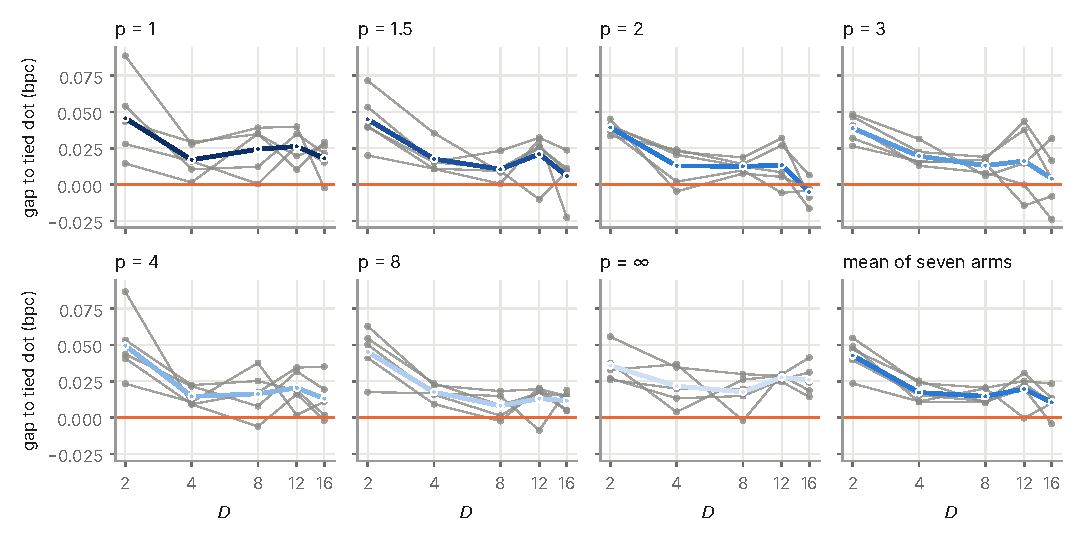
\includegraphics[width=\textwidth]{figures/fig_gap_slopes.pdf}
\caption{Paired gap to the tied dot product against $D$, by arm. Grey lines are the five seeds, the coloured line is the mean, and the orange line is zero.}
\end{figure}

\begin{figure}[h]
\centering
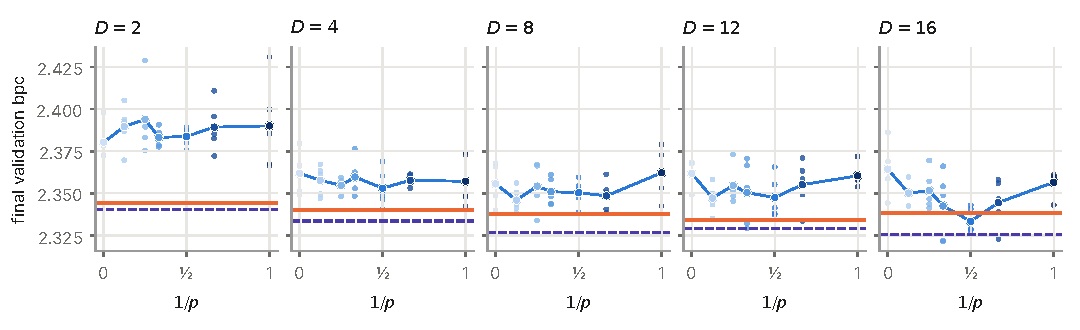
\includegraphics[width=\textwidth]{figures/fig_invp.pdf}
\caption{Final validation bpc against $1/p$ at each head size. Dots are single seeds, large dots are means. The orange line is the tied dot product and the violet dashed line is the untied dot product.}
\end{figure}

\section{Training dynamics at all head sizes}\label{app:training}

\begin{figure}[h]
\centering
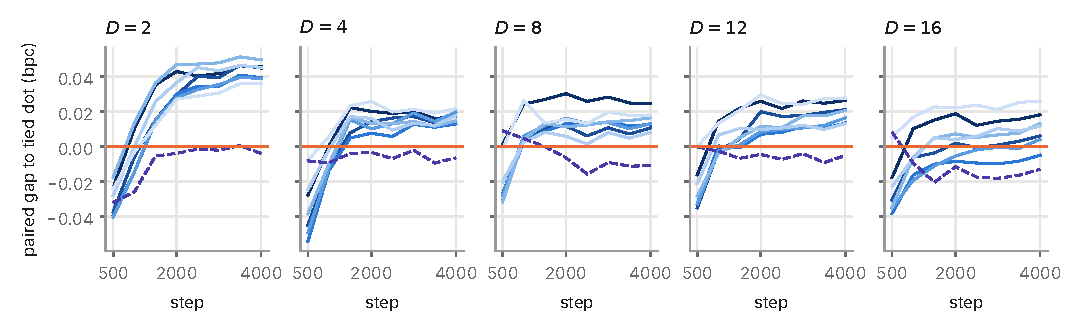
\includegraphics[width=\textwidth]{figures/fig_training_all.pdf}
\caption{Paired gap to the tied dot product during training at every head size, mean of five seeds, by arm (blues as in Figure~\ref{fig:surface}; violet dashed is the untied dot product). The orange line is the tied dot product.}
\end{figure}

\begin{table}[h]
\centering\small
\begin{tabular}{rrr}
\toprule
Step & Cells with an $\ell^p$ arm ahead (of 35) & Mean gap over the 35 cells (bpc) \\
\midrule
500 & 33 & -0.027 \\
1000 & 18 & +0.000 \\
1500 & 4 & +0.013 \\
2000 & 2 & +0.017 \\
2500 & 3 & +0.017 \\
3000 & 2 & +0.019 \\
3500 & 2 & +0.019 \\
4000 & 1 & +0.021 \\
\bottomrule
\end{tabular}

\caption{Number of the 35 cells in which the \Lp{} arm has the lower validation bpc than the tied dot product, and the mean gap over the 35 cells, at each evaluation step.}
\end{table}

\section{Run time}\label{app:time}

\begin{figure}[h]
\centering
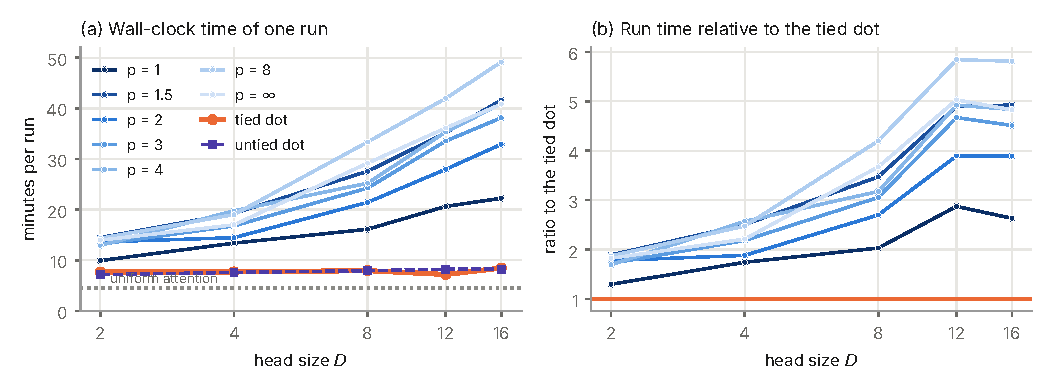
\includegraphics[width=\textwidth]{figures/fig_time.pdf}
\caption{(a) Wall-clock minutes per run against head size. (b) Run time relative to the tied dot product. Tied dot product times vary by about 10\% between runs and periods (7.2 to 8.5 minutes), which accounts for the bump at $D=12$ in (b).}
\end{figure}

\end{document}
